% Physics experiment report
% 29/Oct/2016

\documentclass[a4paper,10pt,notitlepage]{article}

\usepackage{CJKutf8}
\usepackage{amsmath}
\usepackage{indentfirst}
\usepackage{graphicx}
\usepackage{longtable}

\setlength{\parindent}{2em} 

\begin{CJK*}{UTF8}{gbsn}
\begin{document}

\title{弗兰克-赫兹实验报告}
\author{秦光辉\ 9组3号}
\maketitle

\section{实验数据}

\subsection{Hg管的测量}

	第一组实验数据见表一.实验中$U_1 = 1.00V$,$U_3 = 2.00V$,$\theta = 178^\circ$C.
	
	
\begin{center}

	\begin{longtable}{|c|c|c|c|c|c|c|c|c|c|c|}
	\hline
	$U_2$/V & 0.0 & 0.5 & 0.9 & 1.4 & 1.7 & 2.2 & 2.6 & 3.1 & 3.5 & 3.8 \\
	\hline
	$U_{out}$/V & 0.0 & 3.9 & 4.8 & 5.2 & 5.9 & 5.7 & 5.0 & 5.1 & 5.2 & 5.4 \\
	\hline
	\hline
	$U_2$/V & 4.2 & 4.4 & 4.5 & 4.6 & 4.7 & 4.8 & \textbf{4.9} & 5.0 & 5.1 & 5.3 \\
	\hline
	$U_{out}$/V & 6.1 & 7.9 & 8.0 & 8.5 & 9.5 & 10.1 & \textbf{10.2} & 9.6 & 8.6 & 7.9 \\
	\hline
	\hline
	$U_2$/V & 5.5 & 5.6 & 5.8 & 6.0 & 6.3 & 6.6 & 6.9 & 7.2 & 7.5 & 7.8 \\
	\hline
	$U_{out}$/mV & 6.6 & 6.8 & 5.7 & 5.5 & 6.5 & 9.1 & 12.0 & 17.1 & 25.6 & 33.1 \\
	\hline
	\hline
	$U_2$/V & 8.1 & 8.5 & 8.8 & 9.0 & 9.2 & \textbf{9.4} & 9.5 & 9.6 & 9.8 & 10.0 \\
	\hline
	$U_{out}$/mV & 45.0 & 66.5 & 85.2 & 100.7 & 110.2 & \textbf{116.2} & 118.3 & 106.6 & 89.3 & 56.1 \\
	\hline
	\hline
	$U_2$/V & 10.1 & 10.2 & 10.3 & 10.7 & 11.1 & 11.4 & 11.7 & 12.0 & 12.3 & 12.6 \\
	\hline
	$U_{out}$/mV & 42.3 & 31.8 & 25.2 & 11.2 & 10.1 & 14.0 & 19.3 & 29.3 & 45.0 & 56.7 \\
	\hline
	\hline
	$U_2$/V & 13.0 & 13.3 & 13.6 & 13.9 & 14.0 & 14.1 & \textbf{14.2} & 14.3 & 14.5 & 14.7 \\
	\hline
	$U_{out}$/mV & 83.6 & 115 & 143 & 163.6 & 175.1 & 182.1 & \textbf{188.9} & 189.5 & 174.5 & 142.6 \\
	\hline
	\hline
	$U_2$/V & 14.8 & 14.9 & 15.1 & 15.3 & 15.6 & 15.9 & 16.2 & 16.5 & 16.8 & 17.2 \\
	\hline
	$U_{out}$/mV & 124.6 & 112.3 & 81.7 & 52.4 & 26.1 & 16.9 & 19.0 & 27.3 & 37.2 & 60.9 \\
	\hline
	\hline
	$U_2$/V & 17.5 & 17.8 & 18.2 & 18.4 & 18.7 & 18.9 & 19.1 & \textbf{19.2} & 19.3 & 19.5 \\
	\hline
	$U_{out}$/mV & 79.1 & 111.2 & 148.8 & 175.6 & 213.3 & 232.9 & 244.4 & \textbf{247.1} & 239.6 & 226.1 \\
	\hline
	\hline
	$U_2$/V & 19.7 & 20.0 & 20.5 & 20.9 & 21.3 & 21.6 & 21.9 & 22.4 & 22.7 & 23.1 \\
	\hline
	$U_{out}$/mV & 196.2 & 139.2 & 65.4 & 37.2 & 34.6 & 44.2 & 56.1 & 92.0 & 121.7 & 167.4 \\
	\hline
	\hline
	$U_2$/V & 23.3 & 23.6 & 23.7 & 23.8 & 23.9 & 24.0 & 24.1 & \textbf{24.2} & 24.3 & 24.4 \\
	\hline
	$U_{out}$/mV & 196.8 & 239.5 & 255 & 267.3 & 274 & 283.3 & 286.2 & \textbf{290.7} & 289.2 & 285.2 \\
	\hline
	\hline
	$U_2$/V & 24.5 & 24.7 & 24.9 & 25.1 & 25.3 & 25.6 & 25.9 & 26.2 & 26.6 & 27.0 \\
	\hline
	$U_{out}$/mV & 276.4 & 254 & 220.9 & 187.5 & 141.8 & 94.4 & 76.8 & 57.0 & 65.0 & 81.3 \\
	\hline
	\hline
	$U_2$/V & 27.4 & 27.7 & 28.2 & 28.4 & 28.6 & 28.8 & 28.9 & 29.0 & 29.1 & \textbf{29.2} \\
	\hline
	$U_{out}$/mV & 115.9 & 148.1 & 215.7 & 236.3 & 271.3 & 297.9 & 309.6 & 321.2 & 324.2 & \textbf{330.1} \\
	\hline
	\hline
	$U_2$/V & 29.3 & 29.4 & 29.6 & 29.8 & 30.0 & 30.3 & 30.6 & 31.2 &  &\\
	\hline
	$U_{out}$/mV & 329.6 & 324.9 & 308.7 & 286.5 & 264.8 & 205.3 & 164.1 & 110.7 &&  \\
	\hline
	\multicolumn{1}{c}{ } \\
	\caption{Hg管在$U_3$=2.0V的情况下实验数据}
	\end{longtable}
	
\end{center}

	第二组数据见表二.实验中$U_1 = 1.00V$,$U_3 = 2.50V$,$\theta = 179^\circ$C.
	
\begin{center}

	\begin{longtable}{|c|c|c|c|c|c|c|c|c|c|c|}
	\hline
	$U_1$/V & 22.4 & 22.9 & 23.2 & 23.4 & 23.7 & 23.9 & 24.0 & 24.1 & 24.2 & \textbf{24.3} \\
	\hline
	$U_{out}$/mV & 50.9 & 86.4 & 112.7 & 137.8 & 174.3 & 190.7 & 200.8 & 203.5 & 212.2 & \textbf{212.5} \\
	\hline
	\hline
	$U_1$/V & 24.5 & 24.6 & 24.8 & 25.1 & 25.3 & 25.6 & 26.0 & 26.3 & 26.7 & 27.2 \\
	\hline
	$U_{out}$/mV & 207.7 & 199.6 & 172.8 & 148.1 & 109.3 & 82.0 & 46.5 & 39.8 & 39.6 & 51.2 \\
	\hline
	\hline
	$U_1$/V & 27.4 & 27.8 & 28.1 & 28.3 & 28.6 & 28.8 & 28.9 & 29.0 & 29.1 & 29.2 \\
	\hline
	$U_{out}$/mV & 65.0 & 97.5 & 131.6 & 152.6 & 192.6 & 213.7 & 220.1 & 227.3 & 233.2 & 235 \\
	\hline
	\hline
	$U_1$/V & \textbf{29.3} & 29.4 & 29.5 & 29.7 & 29.8 & 30.1 & 30.5 & && \\
	\hline
	$U_{out}$/mV & \textbf{241.4} & 240 & 237 & 231 & 217.3 & 193 & 132.6 &&&  \\
	\hline
	\multicolumn{1}{c}{ } \\
	\caption{Hg管在$U_3$=2.5V的情况下实验数据}
	\end{longtable}

\end{center}

	第三组数据见表三.实验中$U_1 = 1.00V$,$U_3 = 1.50V$,$\theta = 180^\circ$C.
	
\begin{center}

	\begin{longtable}{|c|c|c|c|c|c|c|c|c|c|c|}
	\hline
	$U_0$/V & 22.7 & 23.0 & 23.4 & 23.5 & 23.7 & 23.9 & 24.0 & 24.1 & \textbf{24.2} & 24.3 \\
	\hline
	$U_{out}$/mV & 151.7 & 202.2 & 249 & 256.9 & 282.3 & 309.2 & 321.5 & 325.9 & \textbf{328.2} & 322.7 \\
	\hline
	\hline
	$U_0$/V & 24.4 & 24.6 & 24.9 & 25.2 & 25.6 & 26.0 & 26.3 & 26.6 & 27.0 & 27.4 \\
	\hline
	$U_{out}$/mV & 319.6 & 286.4 & 242.6 & 180.4 & 119 & 92.9 & 90.7 & 99.6 & 122.2 & 166.4 \\
	\hline
	\hline
	$U_0$/V & 27.9 & 28.3 & 28.5 & 28.6 & 28.8 & 29.0 & 29.1 & \textbf{29.2} & 29.3 & 29.4 \\
	\hline
	$U_{out}$/mV & 221.8 & 289 & 320.4 & 331.4 & 356.1 & 376.9 & 382.9 & \textbf{385.7} & 380.7 & 370.9 \\
	\hline
	\hline
	$U_0$/V & 29.6 & 29.9 & 30.3 & 30.6 & 30.8 & 31.2 & &&& \\
	\hline
	$U_{out}$/mV & 357.4 & 323.6 & 231.6 & 192.7 & 170.2 & 145.9 &&&&  \\
	\hline
	\multicolumn{1}{c}{ } \\
	\caption{Hg管在$U_3$=1.5V的情况下实验数据}
	\end{longtable}

\end{center}

	Hg管的F-H图线见图一.

\begin{figure}
	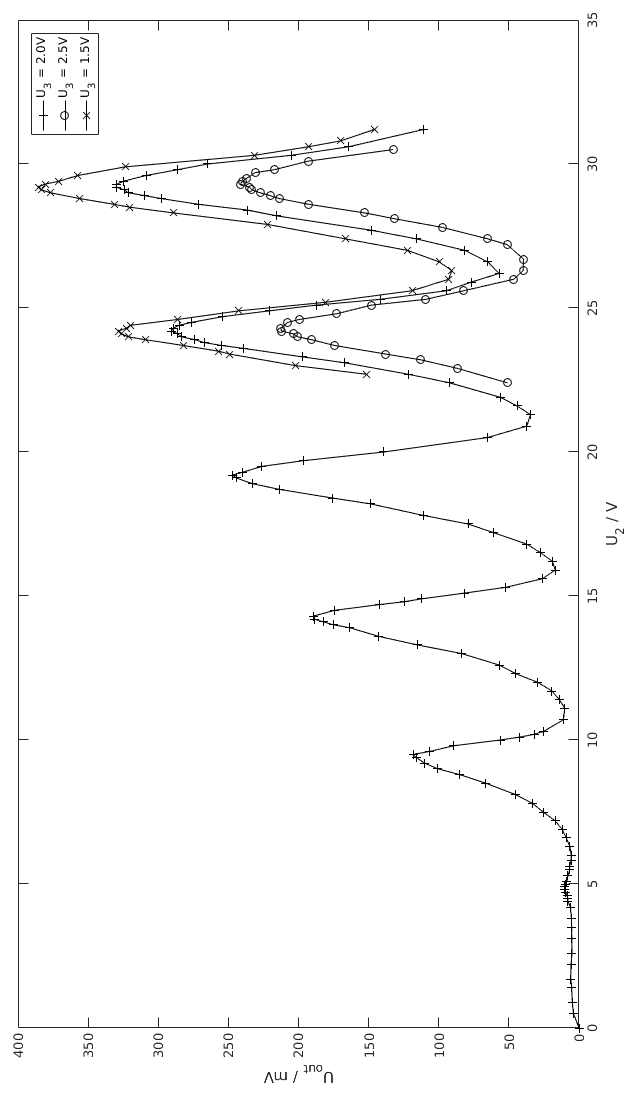
\includegraphics[scale=.7]{fh1.png}
	\caption{Hg管F-H曲线}
\end{figure}

\subsection{Ar的测量}

	实验数据见表四. $V_F$ = 2.6V, $V_{G_1K}$ = 2.4V, $V_{G_2P}$ = 7.5V.
	
\begin{center}

	\begin{longtable}{|c|c|c|c|c|c|c|c|c|c|c|}
	\hline
	$U_{KG_2}$/V & 0.0 & 0.6 & 1.1 & 2.1 & 3.0 & 3.9 & 5.3 & 6.1 & 7.1 & 9.5 \\
	\hline
	$U_{out}$/mV & -3 & -2.9 & -3 & -2.9 & -2.9 & -2.9 & -2.9 & -2.9 & -2.9 & 0.4 \\
	\hline
	\hline
	$U_{KG_2}$/V & 10.0 & 10.7 & 11.1 & 11.6 & 12.0 & 12.5 & 13.0 & 13.5 & 14.0 & 14.6 \\
	\hline
	$U_{out}$/mV & 2.9 & 6.8 & 10.4 & 15.3 & 19.3 & 23.5 & 28.6 & 32.7 & 36.6 & 40.0 \\
	\hline
	\hline
	$U_{KG_2}$/V & 15.0 & 15.5 & 15.7 & 15.9 & 16.1 & 16.3 & 16.5 & \textbf{16.8} & 17.0 & 17.3 \\
	\hline
	$U_{out}$/mV & 41.6 & 43.5 & 43.9 & 44.0 & 44.0 & 44.1 & 44.3 & \textbf{45.0} & 44.2 & 41.9 \\
	\hline
	\hline
	$U_{KG_2}$/V & 17.5 & 17.7 & 18.1 & 18.3 & 18.5 & 19.1 & 19.5 & 20.0 & 20.5 & 21.0 \\
	\hline
	$U_{out}$/mV & 40.9 & 39.5 & 36.6 & 34.7 & 32.6 & 26.8 & 22.0 & 16.7 & 11.4 & 7.9 \\
	\hline
	\hline
	$U_{KG_2}$/V & 21.5 & 22.1 & 22.6 & 23.3 & 23.8 & 24.4 & 25.1 & 25.8 & 26.2 & 26.7 \\
	\hline
	$U_{out}$/mV & 5.2 & 3.9 & 4.8 & 8.9 & 13.6 & 24.4 & 36.0 & 48.9 & 54.9 & 60.2 \\
	\hline
	\hline
	$U_{KG_2}$/V & 26.9 & 27.0 & 27.1 & 27.2 & 27.3 & 27.4 & 27.6 & 27.7 & \textbf{27.9} & 28.0 \\
	\hline
	$U_{out}$/mV & 61.6 & 61.8 & 62.6 & 63.0 & 63.7 & 63.9 & 64.6 & 64.9 & \textbf{65.0} & 64.9 \\
	\hline
	\hline
	$U_{KG_2}$/V & 28.2 & 28.4 & 28.6 & 28.9 & 29.2 & 29.5 & 29.8 & 30.1 & 30.6 & 31.0 \\
	\hline
	$U_{out}$/mV & 64.5 & 64.1 & 63.1 & 61.6 & 59.3 & 55.3 & 51.5 & 46.0 & 37.3 & 28.3 \\
	\hline
	\hline
	$U_{KG_2}$/V & 31.5 & 32.0 & 32.4 & 32.9 & 33.2 & 33.7 & 34.1 & 34.6 & 35.1 & 35.5 \\
	\hline
	$U_{out}$/mV & 18.3 & 10.9 & 6.4 & 2.2 & 0.5 & -0.2 & 0.5 & 3.8 & 8.6 & 16.4 \\
	\hline
	\hline
	$U_{KG_2}$/V & 35.9 & 36.4 & 37.1 & 37.8 & 38.1 & 38.5 & 38.7 & 38.8 & 39.0 & 39.2 \\
	\hline
	$U_{out}$/mV & 24.6 & 35.9 & 54.5 & 69.3 & 73.7 & 79.5 & 82.5 & 82.6 & 84.3 & 86.0 \\
	\hline
	\hline
	$U_{KG_2}$/V & 39.4 & \textbf{39.7} & 39.8 & 40.0 & 40.3 & 40.6 & 40.9 & 41.4 & 41.7 & 42.3 \\
	\hline
	$U_{out}$/mV & 86.7 & \textbf{88.2} & 88.1 & 87.8 & 87.3 & 85.7 & 82.4 & 78.3 & 74.8 & 60.6 \\
	\hline
	\hline
	$U_{KG_2}$/V & 42.7 & 43.1 & 43.6 & 44.0 & 44.5 & 45.2 & 45.5 & 45.8 & 46.6 & 47.4 \\
	\hline
	$U_{out}$/mV & 50.4 & 39.7 & 27.8 & 18.5 & 11.3 & 4.8 & 3.9 & 4.3 & 13.5 & 32.2 \\
	\hline
	\hline
	$U_{KG_2}$/V & 48.1 & 48.7 & 49.0 & 49.6 & 50.1 & 50.6 & 50.7 & 50.9 & 51.1 & 51.3 \\
	\hline
	$U_{out}$/mV & 52.5 & 69.3 & 76.2 & 92.9 & 102.2 & 109.4 & 110.3 & 112.2 & 115 & 116.4 \\
	\hline
	\hline
	$U_{KG_2}$/V & 51.5 & 51.8 & \textbf{52.0} & 52.2 & 52.5 & 52.9 & 53.1 & 53.4 & 53.7 & 54.0 \\
	\hline
	$U_{out}$/mV & 117.8 & 119.7 & \textbf{121.0} & 120.5 & 120 & 118.1 & 115.9 & 112.6 & 107.8 & 103.2 \\
	\hline
	\hline
	$U_{KG_2}$/V & 54.5 & 55.0 & 55.5 & 56.0 & 56.5 & 57.1 & 57.5 & 58.1 & 58.6 & 59.1 \\
	\hline
	$U_{out}$/mV & 91.6 & 73.5 & 67.0 & 54.4 & 41.2 & 31.6 & 26.9 & 23.7 & 25.8 & 33.2 \\
	\hline
	\hline
	$U_{KG_2}$/V & 60.0 & 60.5 & 61.1 & 61.6 & 62.1 & 62.9 & 63.1 & 63.4 & 63.6 & 63.8 \\
	\hline
	$U_{out}$/mV & 53.5 & 67.4 & 84.6 & 98.7 & 112.4 & 131.8 & 135.4 & 141.7 & 145 & 148.3 \\
	\hline
	\hline
	$U_{KG_2}$/V & 64.0 & 64.2 & 64.4 & 64.6 & 64.8 & 65.0 & 65.2 & \textbf{65.5} & 65.7 & 66.0 \\
	\hline
	$U_{out}$/mV & 151.2 & 153.1 & 155.2 & 156.8 & 158.1 & 158.9 & 159.2 & \textbf{159.3} & 158.5 & 156.7 \\
	\hline
	\hline
	$U_{KG_2}$/V & 66.3 & 66.5 & 66.9 & 67.2 & 67.8 & 68.2 & 68.7 & 69.0 & 69.6 & 70.2 \\
	\hline
	$U_{out}$/mV & 152.7 & 150.6 & 144 & 136.2 & 124.2 & 114 & 102.8 & 96.3 & 83.7 & 75.2 \\
	\hline
	\hline
	$U_{KG_2}$/V & 70.6 & 71.1 & 71.6 & 72.1 & 72.7 & 73.2 & 73.7 & 74.3 & 74.7 & 75.0 \\
	\hline
	$U_{out}$/mV & 72.9 & 72.7 & 76.1 & 83.0 & 95.3 & 109.2 & 123.5 & 140.8 & 153.3 & 161.8 \\
	\hline
	\hline
	$U_{KG_2}$/V & 75.3 & 75.5 & 75.8 & 76.0 & 76.2 & 76.3 & 76.4 & 76.5 & 76.7 & 76.9 \\
	\hline
	$U_{out}$/mV & 173.1 & 179.9 & 186.4 & 193 & 197.4 & 201.8 & 204.8 & 207.5 & 212 & 215.5 \\
	\hline
	\hline
	$U_{KG_2}$/V & 77.0 & 77.1 & 77.3 & 77.5 & 77.7 & 77.9 & 78.1 & 78.3 & 78.5 & 78.7 \\
	\hline
	$U_{out}$/mV & 218 & 221.4 & 225.2 & 228.1 & 230.5 & 232.8 & 234.5 & 235.7 & 236.7 & 237.4 \\
	\hline
	\hline
	$U_{KG_2}$/V & \textbf{78.9} & 79.1 & 79.3 & 79.5 & 79.7 & 80.0 & 80.3 & 80.6 & 81.0 & 81.6 \\
	\hline
	$U_{out}$/mV & \textbf{237.7} & 237.5 & 237.6 & 236.2 & 233.9 & 231.9 & 229.8 & 224 & 218.2 & 204.6 \\
	\hline
	\hline
	$U_{KG_2}$/V & 82.0 & 82.5 & 83.0 & 83.6 & 84.1 & 84.9 & &&& \\
	\hline
	$U_{out}$/mV & 197.5 & 188.2 & 182.3 & 177.2 & 176.3 & 181.1 & &&& \\
	\hline
	\multicolumn{1}{c}{ } \\
	\caption{Ar管实验数据}
	\end{longtable}

\end{center}

	Ar管的F-H图线见图二.

\begin{figure}
	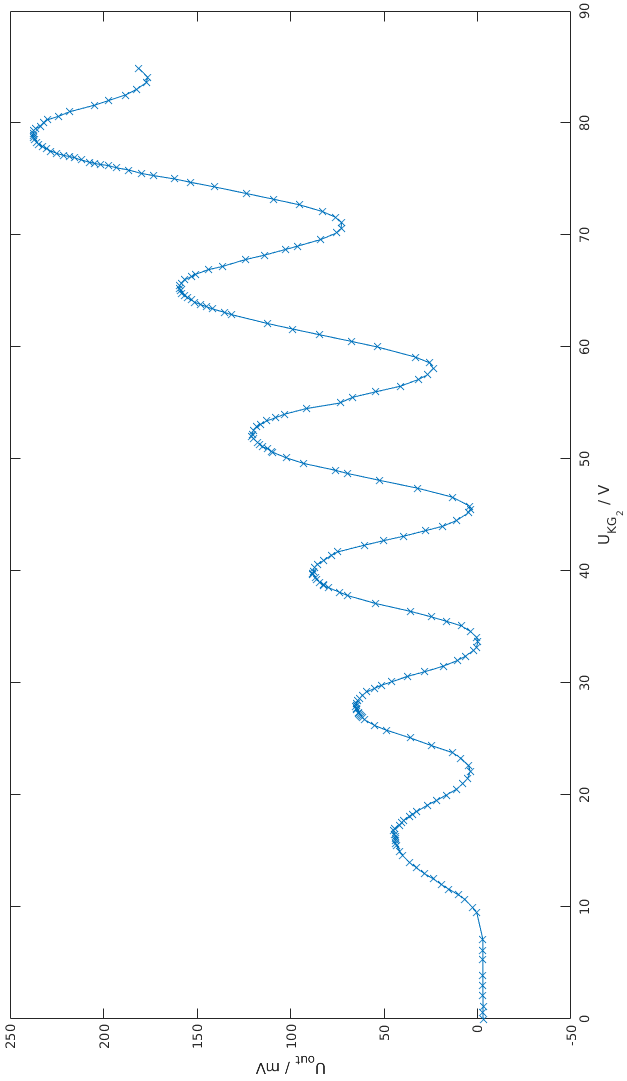
\includegraphics[scale=0.7]{fh2.png}
	\caption{Ar管F-H曲线}
\end{figure}

\subsection{峰值点分析}

	Hg管在$U_1 = 1.00V$,$U_3 = 2.00V$,$\theta = 178^\circ$C实验条件下的峰值点见表五.
	
\begin{center}

	\begin{longtable}{|c|c|c|c|c|c|c|c|c|c|c|}
	\hline
	n & 1 & 2 & 3 & 4 & 5 & 6 \\
	\hline
	$U_{KG_2}$/V & 4.9 & 9.4 & 14.2 & 19.2 & 24.2 & 29.2 \\
	\hline
	\multicolumn{1}{c}{ } \\
	\caption{Hg管峰值点实验数据}
	\end{longtable}

\end{center}

	拟合直线见图三. 可以获得 \\
	
\begin{align*}
	k &= 4.88286V \\
	b &= -0.24V \\
	r &= 0.999814 \\
	\sigma^2 &= \frac{\sum_{i = 1}^{n}(y_i - b - kx_i)^2}{n - 2} = 0.0387 V^2 \\
	\sigma_k &= k \times \sqrt{\frac{1/r^2 - 1}{n - 2}} = 0.047V 
\end{align*}
	
	考虑仪器允差(最小分度为0.1V), 有
	
\begin{align*}
	\sigma_k' &= \sqrt{\sigma_k ^ 2 + \frac{e^2}{3}} = 0.0744V \\
	k &= 4.88 \pm 0.08 V
\end{align*}

	可见Hg原子第一激发态的能量为$4.88 \pm 0.08$V. \\
	
\begin{figure}
	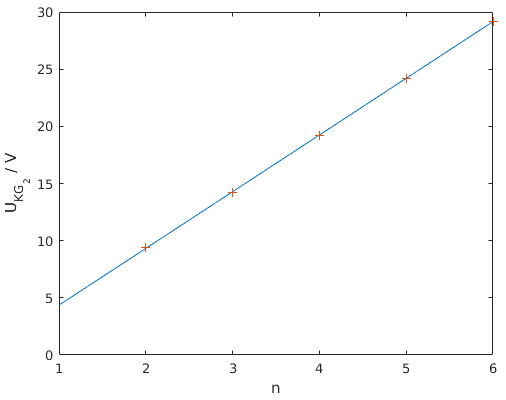
\includegraphics[scale=0.76]{fh3.png}
	\caption{Hg管$U_{KG_2}$和峰值线性拟合图线}
\end{figure}

	Ar管在$V_F$ = 2.6V, $V_{G_1K}$ = 2.4V, $V_{G_2P}$ = 7.5V实验条件下的峰值点见表六.
	
\begin{center}

	\begin{longtable}{|c|c|c|c|c|c|c|c|c|c|c|}
	
	\hline
	n & 1 & 2 & 3 & 4 & 5 & 6 \\
	\hline
	$U_{KG_2}$/V & 16.8 & 27.9 & 39.7 & 52.0 & 65.5 & 78.9 \\
	\hline

	\multicolumn{1}{c}{ } \\
	\caption{Ar管峰值点实验数据}
	\end{longtable}

\end{center}

	拟合直线见图四. 可以获得 
	
\begin{align*}
	k &= 12.4457 V \\
	b &= 3.24V \\
	r &= 0.9999284 \\
	\sigma^2 &= \frac{\sum_{i = 1}^{n}(y_i - b - kx_i)^2}{n - 2} = 1.02086 V^2 \\
	\sigma_k &= k \times \sqrt{\frac{1/r^2 - 1}{n - 2}} = 0.242V 
\end{align*}
	
	考虑仪器允差(最小分度为0.1V), 有
	
\begin{align*}
	\sigma_k' &= \sqrt{\sigma_k ^ 2 + \frac{e^2}{3}} = 0.249V \\
	k &= 12.4 \pm 0.3 V
\end{align*}

	可见Ar原子第一激发态的能量为$12.4 \pm 0.3$V. \\
	
\begin{figure}
	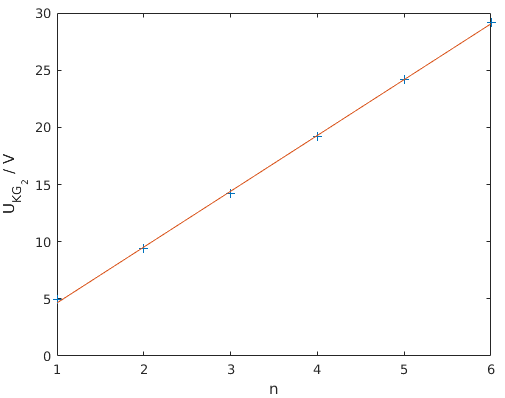
\includegraphics[scale=0.76]{fh4.png}
	\caption{Ar管$U_{KG_2}$和峰值线性拟合图线}
\end{figure}

\section{思考题}

	根据图一来看, 当反向电压增大的时候, 输出电压$U_{out}$会减小, 反之则增大. 如果仅考虑最后两个峰值, 我们可以看出出现极值的$U_2$几乎没有变化(相差不超过0.1V). \\
	
	当反向电压增大的时候, 通过Hg管到达P极板的电子数量会减小, 电流会随之减弱, 自然输出电压会减小.
	
\section{分析与讨论}

\subsection{实验中测得的各种曲线有什么主要特征?如何理解?}

	图中测得的图一和图二的曲线呈现周期性的峰值和谷底, 这来源于电子和气体分子之间的碰撞. 以Hg原子为例, 加速电压增大的时候, 电子的动能也随之增大. 当电子的能量达到4.9V时, 自由电子恰好足以激发Hg到达其第一激发态, 这样很多电子就被Hg原子吸收了部分能量而不足以到达P极板. 我们在实验中看到当加速电压到达4.9V之后, 电流迅速下降, 就是这个原因. 当电压达到9.8V左右的时候, 自由电子可以和Hg原子发生两次非弹性碰撞, 这样就形成了第二个峰值. 如此往复就可以看到周期性的上升和下降. \\
	
	而由于加速电压的增大, 越来越多的电子可以克服反向电压到达P极板, 所以我们在实验中可以看到输出电压的高峰的电压值一直在单调上升. 
	
\subsection{分析测量第一激发电位时误差的主要来源}

\begin{enumerate}
	\item 最主要的误差来源是输出电压值的不稳定. 由于输出电压一直在跳跃, 我们很难读到一个稳定的电压值, 这样每次的数据记录都会有一定的主观性, 无法做到相对客观.
	\item 电压值的衰减和变化是一个重要的误差来源. 在实验中, 由于一些我无法理解的原因, 输出电压不但在跳跃, 而且在一段相对较长的时间内, 其示数会上升或下降. 实验几乎无法重复. 而在测量Ar的特征曲线的时候, 实验仪器曾经有一次故障, 重启之后在相同的加速电压值附近出现了不同的示数. 我猜测这是因为管内达到平衡态需要相当长时间的原因造成的. 如果等待时间足够长, 应该可以获得理想数据.
	\item Hg原子的第一个峰值数值很小, 很难读取. 在图线上可以看到这个峰值特别低. 在低电压下, 电压表的跳跃对实验影响非常大, 非常难以测准.
\end{enumerate}

\section{思考和感悟}

	这个实验是一个非常有名的实验, 它第一次验证了原子的能级分布. 但是其实这个实验的原理并不复杂, 甚至作为本科生的我也能掌握. 虽然这个实验的数据很多, 但是操作也不复杂, 最后得到的图线也非常理想. 我认识到简单的实验也可以反映深刻的原理, 非常基础的物理理论也可能在这样简单的实验中体现出来. 

\end{CJK*}
\end{document}
